\documentclass[tikz,border=3pt]{standalone}
\usetikzlibrary{arrows.meta,shapes.geometric}

\begin{document}
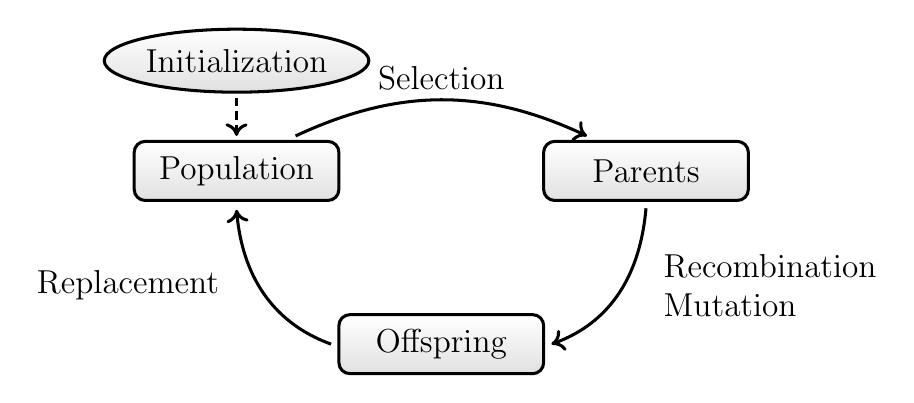
\begin{tikzpicture}[
    font=\large,
    >={To[length=1.6mm,width=2.8mm]},
    stage/.style={
        rectangle, rounded corners=0.14cm, draw, line width=1.1pt,
        top color=white, bottom color=black!12,
        minimum width=2.6cm, minimum height=0.75cm, inner sep=2pt},
    start/.style={
        ellipse, draw, line width=1.1pt,
        top color=white, bottom color=black!12,
        minimum width=3.3cm, minimum height=0.8cm, inner sep=1pt},
    cycle/.style={->, line width=1.1pt},
]

% ---------------- Nodes ----------------
\node[start] (init) at (0,3.6)   {Initialization};
\node[stage] (pop)  at (0,2.2)   {Population};
\node[stage] (par)  at (5.2,2.2) {Parents};
\node[stage] (off)  at (2.6,0)   {Offspring};

% ---------------- Initialization ----------------
\draw[cycle, dash pattern=on 3pt off 2pt]
    ([yshift=-0.05cm]init.south) -- ([yshift=0.05cm]pop.north);

% ---------------- Selection ----------------
\draw[cycle] ([xshift=0.75cm,yshift=0.05cm]pop.north)
    to[out=25,in=155]
    node[above, pos=0.5] {Selection}
    ([xshift=-0.75cm,yshift=0.05cm]par.north);

% ---------------- Recombination / Mutation ----------------
\draw[cycle] ([yshift=-0.08cm]par.south)
    to[out=-95,in=20] ([xshift=0.08cm]off.east);
\node[align=left, anchor=west] at (5.3,0.75) {Recombination\\Mutation};

% ---------------- Replacement ----------------
\draw[cycle] ([xshift=-0.08cm]off.west)
    to[out=160,in=-85] ([yshift=-0.1cm]pop.south);
\node[anchor=east] at (-0.1,0.75) {Replacement};

\end{tikzpicture}
\end{document}
